% !TEX root= ../main.tex
\section{Unary NAND-clauses in graph theories}
\label{sec:Unary NAND-clauses in graph theories}
We will to use the fact that some binary NAND-clauses are not binary-derivable to show that some \textit{unary} NAND-clauses are not binary-derivable.

We use our graph from Figure~\ref{fig:open_door} to make the following, bigger graph:\par
\begin{figure}[!h]
  \centering
  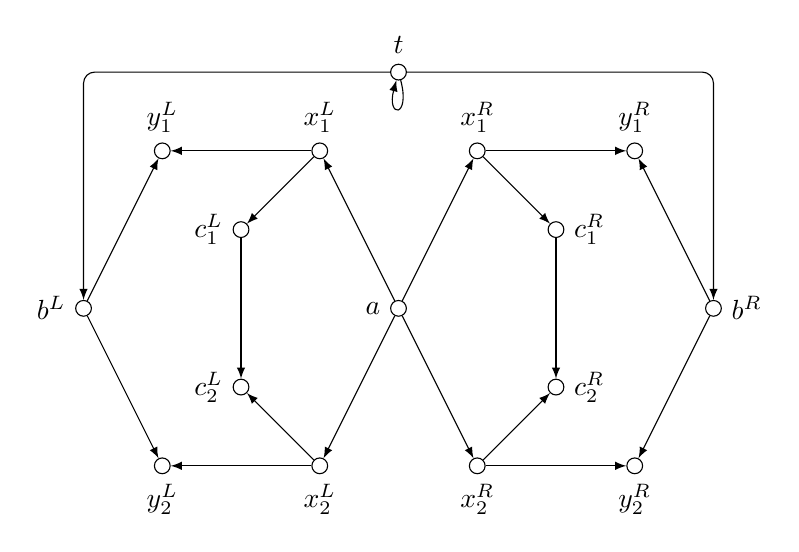
\begin{tikzpicture}
    [
    point/.style={circle,draw,inner sep=0pt,minimum size=2mm}
    ]
    \node (t) at (4,5) [point,label=above:$t$] {};
    \node (a) at (4,2) [point,label=left:$a$] {};
    \node (lx1) at (3,4) [point,label=above:$x^L_1$] {};
    \node (lx2) at (3,0) [point,label=below:$x^L_2$] {};
    \node (lb) at (0,2) [point,label=left:$b^L$] {};
    \node (ly1) at (1,4) [point,label=above:$y^L_1$] {};
    \node (ly2) at (1,0) [point,label=below:$y^L_2$] {};
    \node (lc1) at (2,3) [point,label=left:$c^L_1$] {};
    \node (lc2) at (2,1) [point,label=left:$c^L_2$] {};
    \draw [-latex] (a) to (lx1);
    \draw [-latex] (a) to (lx2);
    \draw [-latex] (lb) to (ly1);
    \draw [-latex] (lb) to (ly2);
    \draw [-latex] (lx1) to (ly1);
    \draw [-latex] (lx1) to (lc1);
    \draw [-latex] (lx2) to (ly2);
    \draw [-latex] (lx2) to (lc2);
    \draw [-latex] (lc1) to (lc2);
    \node (rx1) at (5,4) [point,label=above:$x^R_1$] {};
    \node (rx2) at (5,0) [point,label=below:$x^R_2$] {};
    \node (rb) at (8,2) [point,label=right:$b^R$] {};
    \node (ry1) at (7,4) [point,label=above:$y^R_1$] {};
    \node (ry2) at (7,0) [point,label=below:$y^R_2$] {};
    \node (rc1) at (6,3) [point,label=right:$c^R_1$] {};
    \node (rc2) at (6,1) [point,label=right:$c^R_2$] {};
    \draw [-latex] (a) to (rx1);
    \draw [-latex] (a) to (rx2);
    \draw [-latex] (rb) to (ry1);
    \draw [-latex] (rb) to (ry2);
    \draw [-latex] (rx1) to (ry1);
    \draw [-latex] (rx1) to (rc1);
    \draw [-latex] (rx2) to (ry2);
    \draw [-latex] (rx2) to (rc2);
    \draw [-latex] (rc1) to (rc2);

    \draw [-latex, rounded corners] (t) -| (lb);
    \draw [-latex, rounded corners] (t) -| (rb);
    \draw [-latex, loop below] (t) to (t);
  \end{tikzpicture}
  \caption{}
  \label{fig:double_open_door}
\end{figure}
\FloatBarrier
The above graph contains two copies of the graph from Figure~\ref{fig:open_door}, only connected by their shared vertex $a$ and the vertex $t$ that has both $b^L$ and $b^R$ in its neighborhood.
We will refer to the two copies as the left component and the right component, with $a$ being in both and $t$ being in none.

The rest of this section will show that the unary NAND-clause $\ol{a}$ is provable, but not binary derivable.

Both $\ol{ab^L}$ and $\ol{ab^R}$ can be proven in the exact the same manner as $\ol{ab}$ was proven earlier in Figure~\ref{fig:v3_counter_proof}.
This makes the proof of $\ol{a}$ trivial:\par
\begin{figure}[!h]
  \centering
  \begin{prooftree*}
    \Hypo{\ol{t}}
    \Hypo{\dots}
    \Infer[]1{\ol{ab^L}}
    \Hypo{\dots}
    \Infer[]1{\ol{ab^R}}
    \Infer[right label=$tb^Lb^R$]3{\ol{a}}
  \end{prooftree*}
  \caption{}
  \label{fig:unary_nand_proof}
\end{figure}
To show that $\ol{a}$ is not binary-derivable, we will first prove the following lemma:
\begin{lemma}
  Based on the graph in Figure~\ref{fig:double_open_door}, the only binary-derivable, non-axiomatic binary NAND-clause containing the atom $a$ is $\ol{at}$.
\end{lemma}

\begin{proof}
We prove this lemma by inducing over the proof length of some binary NAND-clause $\ol{a\gamma}$ and show that $\gamma$ always has to equal either some $x$-vertex or the $t$-vertex.

In the base case, the proof length is 1, so all the clauses in the premise must be axiomatic.
That includes at least one clause containing $a$ and at least one clause containing $\gamma$.
Figure~\ref{fig:nand_base_case} illustrates the situation.\par
\begin{figure}[!h]
  \centering
  \begin{prooftree*}
    \Hypo{\ol{ax^K_i}}
    \Hypo{\ol{\gamma y^K_i}}
    \Hypo{\ol{\gamma c^K_i}}
    \Infer[right label=$x^K_iy^K_ic^K_i$]3{\ol{a\gamma}}
  \end{prooftree*}
  \caption{}
  \label{fig:nand_base_case}
\end{figure}
\FloatBarrier
The only axiomatic NAND-clauses containing $a$ are on the form $\ol{ax^K_i}$ ($K$ being either $L$ or $R$ and $i$ either 1 or 2).
The OR-clause used must be therefore be the corresponding $x^K_iy^K_ic^K_i$, being the only OR-clause containing $x^K_i$.
Since the OR-clause is of length 3, the premise must contain two other clauses and they must have the following form in order to give us $\ol{a \gamma}$ in the conclusion:
$\ol{\gamma y^K_i},\ol{\gamma c^K_i}$.
The only pairs of axioms that matches this description are the ones where $\gamma = x^K_i$.
With a proof length of 1, we are thus not able to prove binary NAND-clauses containing $a$ that are non-axiomatic.

For the inductive step, we assume that if a binary proof of length $k-1$ or less conclude with a binary non-axiomatic NAND-clause containing $a$ then the clause in question is $\ol{at}$, and will show the same holds for any binary proof of length $k$.

Suppose we have a proof of length $k$ that concludes with some binary NAND-clause $\ol{a\gamma}$;
like in the base case, we have that the premise of the last proof step must contain at least one NAND-clause containing $a$ and at least one containing $\gamma$.
Because of our induction hypothesis, we have that the only available NAND-clauses containing $a$ are $\ol{at}$ and the four axioms on the form $\ol{ax^K_i}$.

Let us first consider the case where some $\ol{ax^K_i}$ is in the premise.
This case will be very similar to the base case.
Like in the base case, the only applicable OR-clause is the corresponding $x^K_iy^K_ic^K_i$, so the premise contains two additional NAND-clauses, one containing $y^K_i$ and one containing $c^K_i$.
Because of our induction hypothesis, those two cannot contain $a$, so either both contain $\gamma$ or one is unary while the other contain $\gamma$.
Neither $\ol{y^K_i}$ nor $\ol{c^K_i}$ is provable\todo{show assignments}, so they both have to contain $\gamma$.
Thus, like in the base case, the two additional NAND-clauses must be on the form $\ol{\gamma y^K_i},\ol{\gamma c^K_i}$.
Except for the case where $\gamma = x^K_i$, the only $\gamma$-assignment that makes both of these NAND-clauses provable is $\gamma = t$\todo{show assignments}, giving us $\ol{at}$ in the conclusion.

The other case is where $\ol{at}$ appears in the premise.
Figure~\ref{fig:nand_inductive_step} illustrates this situation.\par
\begin{figure}[!h]
  \centering
  \begin{prooftree*}
    \Hypo{\ol{at}}
    \Hypo{\dots}
    \Infer[]1{\ol{\gamma b^L}}
    \Hypo{\dots}
    \Infer[]1{\ol{\gamma b^R}}
    \Infer[right label=$tb^Lb^R$]3{\ol{a\gamma}}
  \end{prooftree*}
  \caption{}
  \label{fig:nand_inductive_step}
\end{figure}
In order to ``strip off'' the $t$, the only applicable OR-clase is $tb^Lb^R$, again giving us three NAND-clauses in the premise.
The two additional clauses must contain $b^L$ and $b^R$, respectively.
None of them are provably false\todo{show assignments}, and none of them can contain $a$ because of induction hypothesis, so they both must contain some $\gamma$.
The only $\gamma$-assignment applicable such that both $\ol{\gamma b^L}$ and $\ol{\gamma b^R}$ is provable is, again, $\gamma = t$\todo{show assignments}, giving us $\ol{at}$ in the conclusion.

The only binary-provable, non-axiomatic, binary NAND-clause containing $a$ is therefore $\ol{at}$.
\end{proof}

It is now easy to show that $\ol{a}$ is indeed not binary-provable.
Suppose we have a binary proof concluding with $\ol{a}$.
There must exists a NAND-clause in the immediate premise of this conclusion containing either $\ol{at}$ or some $\ol{ax^K_i}$.
Because of the above proof, we know that no other binary NAND-clauses containing $a$ are binary-derivable.

In the case with $\ol{at}$,the OR-clause $tb^Lb^R$ must be used.
Now, in order to prove $\ol{a}$, the premise must contain either $\ol{a b^L}$ or $\ol{b^L}$, but $\ol{a b^L}$ is not binary-derivable and $\ol{b^L}$ is not even provable.

In the case with $\ol{ax^K_i}$ in the premise, we get the same problem;
The only applicable OR-clause is $x^K_iy^K_ic^K_i$, but neither $\ol{a y^K_i}$ nor $\ol{y^K_i}$ is binary-derivable.

We therefore get that no binary proof exists with $\ol{a}$ as its conclusion, making $\ol{a}$ provable, but not binary-derivable.

We will use this result in the following chapter to show that there exist inconsistent graphs such that the inconsistency is not binary-derivable.
